\section[两个角动量的耦合]{两个角动量的耦合} \label{sec:07.07} % 
% \makebox[5em][s]{} % 短题目拉间距

电子的自旋角动量与轨道角动量相加成总角动盘($\S$\ref{sec:07.02})是角动量耦合的一个实例.本节讨论一般的角动量耦合问题.

设$\boldsymbol{J}_{1}$和$\boldsymbol{J}_{2}$是属于不同自由度的角动量算符,它们互相对易:
\begin{empheq}{equation}\label{eq77.1}
	[J_{1\alpha},J_{2\beta}]=0,\quad \alpha,\beta = x,y,z
\end{empheq}
而又各自满足角动量对易式:
\begin{empheq}{equation}\label{eq77.2}
	\boldsymbol{J}_{1}\times\boldsymbol{J}_{1}=i\hbar\boldsymbol{J}_{1},\quad \boldsymbol{J}_{2}\times\boldsymbol{J}_{2}=i\hbar\boldsymbol{J}_{2}
\end{empheq}
因此必然有
\begin{empheq}{equation}\label{eq77.3}
	[\boldsymbol{J}_{1}^{2},\boldsymbol{J}_{1}]=0,\quad [\boldsymbol{J}_{2}^{2},\boldsymbol{J}_{2}]=0
\end{empheq}
以$\boldsymbol{J}$表示$\boldsymbol{J}_{1},\boldsymbol{J}_{2}$之和,即
\begin{empheq}{equation}\label{eq77.4}
	\boldsymbol{J}=\boldsymbol{J}_{1}+\boldsymbol{J}_{2}
\end{empheq}
则
\begin{empheq}{equation}\label{eq77.5}
	\boldsymbol{J}^{2}=\boldsymbol{J}_{1}^{2}+\boldsymbol{J}_{2}^{2}+2\boldsymbol{J}_{1}\cdot\boldsymbol{J}_{2}
\end{empheq}
由\eqref{eq77.1}式,易知
\begin{empheq}{align}
	\boldsymbol{J}_{1}\cdot\boldsymbol{J}_{2}&=\boldsymbol{J}_{2}\cdot\boldsymbol{J}_{1}	\label{eq77.6}\\
	\boldsymbol{J}_{1}\times\boldsymbol{J}_{2}&=-\boldsymbol{J}_{2}\times\boldsymbol{J}_{1}	\label{eq77.7}
\end{empheq}
因此
\eqlong
\begin{empheq}{align}\label{eq77.8}
	\boldsymbol{J}\times\boldsymbol{J}&=\boldsymbol{J}_{1}\times\boldsymbol{J}_{1}+\boldsymbol{J}_{2}\times\boldsymbol{J}_{2}+\boldsymbol{J}_{1}\times\boldsymbol{J}_{2}+\boldsymbol{J}_{2}\times\boldsymbol{J}_{1}	\nonumber\\
	&=i\hbar\boldsymbol{J}_{1}+i\hbar\boldsymbol{J}_{2}=i\hbar\boldsymbol{J}
\end{empheq}\eqnormal
因此$\boldsymbol{J}$也是角动量容易证明
\eqshort
\begin{empheq}{equation}\label{eq77.9}
	[\boldsymbol{J}^{2},\boldsymbol{J}]=0
\end{empheq}\eqnormal
利用\eqref{eq77.3}式容易证明
\begin{empheq}{equation}\label{eq77.10}
	[\boldsymbol{J}_{1}^{2},\boldsymbol{J}]=0,\quad [\boldsymbol{J}_{2}^{2},\boldsymbol{J}]=0
\end{empheq}
因此,$\boldsymbol{J}_{1}^{2},\boldsymbol{J}_{2}^{2},\boldsymbol{J}^{2},J_{z}$互相对易,可以选作力学量完全集.
\pskip

$\S$\ref{sec:04.07}中关于角动量的一般理论对于这里的$\boldsymbol{J}_{1},\boldsymbol{J}_{2}$和$\boldsymbol{J}$均可适用.以$\varPsi_{j_{1}m_{1}}$或$|j_{1}m_{1}\rangle$表示$(\boldsymbol{J}_{1}^{2},J_{1z})$共同本征态,即设
\eqlong
\begin{empheq}{equation}\label{eq77.11}
	\begin{aligned}
		\boldsymbol{J}_{1}^{2}\varPsi_{j_{1}m_{1}} &=j_{1}(j+1)\hbar^{2}\varPsi_{j_{1}m_{1}}	\\
		J_{1z}\varPsi_{j_{1}m_{1}} &=m_{1}\hbar\varPsi_{j_{1}m_{1}},\quad m_{1}=j_{1},j_{1}-1,\cdots(-j_{1})
	\end{aligned}
\end{empheq}
按照$\S$\ref{sec:04.07},升降算符的作用结果是
\eqllong
\begin{empheq}{equation}\label{eq77.12}
	(J_{1x}\pm iJ_{1y})\varPsi_{j_{1}m_{1}}=\hbar\sqrt{(j_{1}\pm m_{1}+1)(j_{1}\mp m_{1})}\varPsi_{j_{1}m_{1}\pm 1}
\end{empheq}
类似地,以$\varPsi_{j_{2}m_{2}}$或$|j_{2}m_{2}\rangle$表示$(\boldsymbol{J}_{2}^{2},J_{2z})$共同本征态,也有类似于\eqref{eq77.11}式、\eqref{eq77.12}式的公式,不再一一写出.
\pskip

$(\boldsymbol{J}_{1}^{2},\boldsymbol{J}_{2}^{2},\boldsymbol{J}^{2},J_{z})$共同本征态记为$\varPsi_{j_{1}j_{2}jM}$或$|j_{1}j_{2}jM\rangle$,相应于本征值
\begin{empheq}{equation}\label{eq77.13}
	\begin{aligned}
		&\boldsymbol{J}_{1}^{2}=j_{1}(j_{1}+1)\hbar^{2},\quad &\boldsymbol{J}_{2}^{2}=j_{2}(j_{2}+1)\hbar^{2}			\\
		&\boldsymbol{J}^{2}=j(j+1)\hbar^{2},\quad 
		&J_{z}=M\hbar,M=j,j-1,\cdots,(-j)
	\end{aligned}
\end{empheq}\eqlong
首先要解决的问题是,当$j_{1}$与$j_{2}$给定后,$j$有哪些可能取值.其次的问题是,$\varPsi_{j_{1}j_{2}jM}$态和$\varPsi_{j_{1}m_{1}}$及$\varPsi_{j_{2}m_{2}}$态是什么关系.按照$\S$\ref{sec:07.02}的经验,$\varPsi_{j_{1}j_{2}jM}$显然可以表示成
\begin{empheq}{equation}\label{eq77.14}
	\varPsi_{j_{1}j_{2}jM}=\sum_{m_{1}}\sum_{m_{2}}C(j,M,m_{1},m_{2})\varPsi_{j_{1}m_{1}}\varPsi_{j_{2}m_{2}}
\end{empheq}\eqnormal
由于$J_{z}=J_{1z}+J_{2z}$,显然有
\begin{empheq}{equation}\label{eq77.15}
	J_{z}\varPsi_{j_{1}m_{1}}\varPsi_{j_{2}m_{2}}=(m_{1}+m_{2})\hbar\varPsi_{j_{1}m_{1}}\varPsi_{j_{2}m_{2}}
\end{empheq}
因此\eqref{eq77.14}式中只包含$m_{1}+m_{2}=M$的项.给定$j_{1},j_{2}$后,$m_{1}$共有$(2j_{1}+1)$种取值(依次相差1),$m_{2}$共有$(2j_{2}+1)$种取值(依次相差1),故\eqref{eq77.14}式右端最多有$(2j_{1}+1)(2j_{2}+1)$种独立项,最多能组成同样数目的独立的$\varPsi_{j_{1}j_{2}jM}$.其中对于某个$j$值,相应的$M$值有$(2j+1)$种,即
\begin{empheq}{equation*}
	M=j,j-1,\cdots,(-j)
\end{empheq}
由于$M$值只能依次相差1,所以$j$也只能依次相差1.$M$的最大值显然是$(j_{1}+j_{2})$,这也就是$j$的最大值.因此,$j$的可能取值为
\begin{empheq}{equation*}
	j=j_{1}+j_{2},j_{1}+j_{2}-1,\cdots,j_{min}
\end{empheq}
由此可知,独立的$\varPsi_{j_{1}j_{2}jM}$总数为
\begin{empheq}{equation*}
	N=\sum_{j}(2j+1)=(j_{1}+j_{2}+j_{min}+1)(j_{1}+j_{2}-j_{min}+1)
\end{empheq}
上式应等于$(2j_{1}+1)(2j_{2}+1)$,为此必须$j_{min}=|j_{1}-j_{2}|$.因此,$j$的取值为
\begin{empheq}{equation}\label{eq77.16}
	\boxed{j=j_{1}+j_{2},j_{1}+j_{2}-1,\cdots,|j_{1}-j_{2}|}
\end{empheq}
量子数$j_{1},j_{2}$,$j$之间的这种关系常被形象地称为三角形条件,记为$\Delta(j_{1}j_{2}j)$,或用图\ref{fig.7-4}表示,但必须记住,$j$是量子化的,所以图中$j_{1},j_{2}$的夹角也必须是量子化的,以保证\eqref{eq77.16}式成立.

\begin{wrapfigure}[8]{r}{7em}
	\centering
	\small
	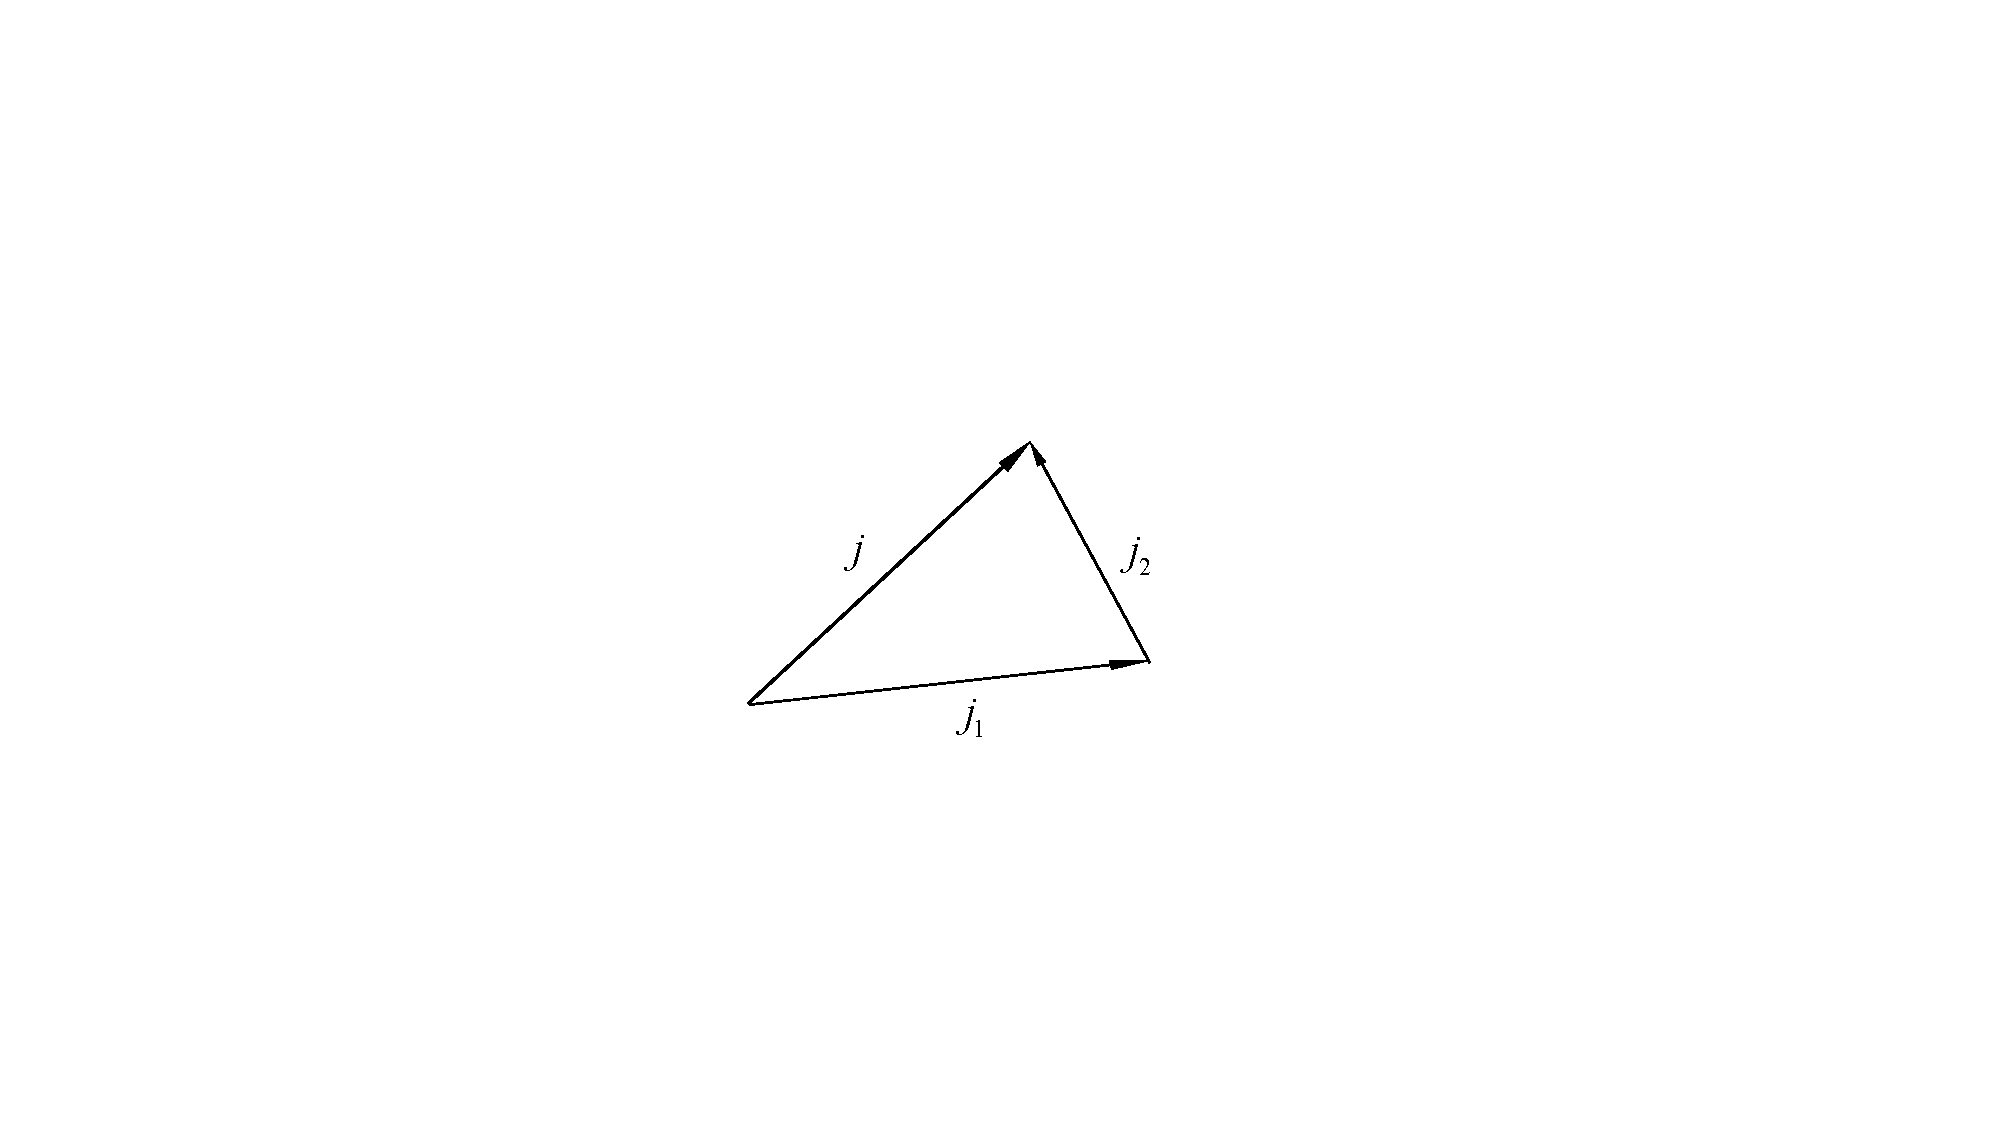
\includegraphics[width=3cm,clip]{QM file/figure/7-4}
	\caption{}\label{fig.7-4}
\end{wrapfigure}

\eqref{eq77.14}式中的系数$C(j,M,m_{1},m_{2})$称为C.G.(Clebsch-Gordan)系数,也称矢耦系数,有关理论和公式相当复杂,从略.如采用狄拉克态矢量符号,$\varPsi_{j_{1}m_{1}},\varPsi_{j_{2}m_{2}}$记成$|j_{1}m_{1},j_{2}m_{2}\rangle$,$\varPsi_{j_{1}j_{2}jM}$记成$|j_{1}j_{2}jM\rangle$,简写成$|jM\rangle$.给定$j_{1},j_{2}$后,我们就有一个$(2j_{1}+1)(2j_{2}+1)$维态矢量空间.如以$|j_{1}m_{1},j_{2}m_{2}\rangle$作为基矢,相应的表象称为非耦合表象;如以$|jM\rangle$作为基矢,相应的表象称为耦合表象.利用恒等变换公式
\begin{empheq}{equation}\label{eq77.17}
	\sum_{m_{1}}\sum_{m_{2}}|j_{1}m_{1},j_{2}m_{2}\rangle \langle j_{1}m_{1},j_{2}m_{2}|=1
\end{empheq}
将$|jM\rangle$在非耦合表象中展开成
\begin{empheq}{equation}\label{eq77.18}
	|jM\rangle=\sum_{m_{1}}\sum_{m_{2}}|j_{1}m_{1},j_{2}m_{2}\rangle \langle j_{1}m_{1},j_{2}m_{2}|jM\rangle 
\end{empheq}
与\eqref{eq77.14}式比较,易见
\begin{empheq}{equation}\label{eq77.19}
	C(jM,m_{1}m_{2})=\langle j_{1}m_{1}j_{2}m_{2}|jM \rangle 
\end{empheq}
显然C.G.系数就是联系两种表象的么正矩阵的矩阵元.

C.G.系数应用极广,有许多类型的C.G.系数表可供查阅.$j_{2}=\frac{1}{2}$和1时C.G.系数如表\ref{lab.7-1},表\ref{lab.7-2}所示.请将$\S$\ref{sec:07.02}中结果与表\ref{lab.7-1}对照$\bigg(j_{1}=l,j_{2}=\frac{1}{2},M=m+\frac{1}{2}\bigg)$


\begin{table}[!h]
	\begin{center}
		\caption{C.G.系数$\langle j_{1}m_{1}j_{2}m_{2}|jM\rangle\bigg(j_{2}=\dfrac{1}{2},m_{1}=M-m_{2}\bigg)$}
		\label{lab.7-1}
		\setlength{\tabcolsep}{8mm}	% 调节表格尺寸
		%\resizebox{h-length}{v-length}{text}
		\begin{tabular}{c|c|c}
			\toprule[1pt]
			\multirow{2}{*}{	} & \multirow{2}{*}{$m_{2}=\frac{1}{2}$} & \multirow{2}{*}{$m_{2}=-\frac{1}{2}$}	\\ 
			 & & \\
			\hline
			\multirow{2}{*}{}
			\multirow{2}{*}{$j=j_{1}+\frac{1}{2}$} & \multirow{2}{*}{$\sqrt{\frac{j_{1}+M+\frac{1}{2}}{2j_{1}+1}}$} & \multirow{2}{*}{$\sqrt{\frac{j_{1}-M+\frac{1}{2}}{2j_{1}+1}}$}	\\ 
			& & \\
			\hline
			\multirow{2}{*}{$j=j_{1}-\frac{1}{2}$} & \multirow{2}{*}{$-\sqrt{\frac{j_{1}-M+\frac{1}{2}}{2j_{1}+1}}$} & \multirow{2}{*}{$\sqrt{\frac{j_{1}+M+\frac{1}{2}}{2j_{1}+1}}$}	\\ 
			& & \\
			\bottomrule[1pt]
		\end{tabular}
	\end{center}
\end{table}

\begin{table}[!h]
	\begin{center}
		\caption{C.G.系数$\langle j_{1}m_{1}j_{2}m_{2}|jM\rangle\bigg(j_{2}=1,m_{1}=M-m_{2}\bigg)$}
		\label{lab.7-2}
		%\setlength{\tabcolsep}{3mm}	% 调节表格尺寸
		%\resizebox{h-length}{v-length}{text}
		\begin{tabular}{c|c|c|c}
			\toprule[1pt]
			\multirow{2}{*}{	}& \multirow{2}{*}{$m_{2}=1$} & \multirow{2}{*}{$m_{2}=0$} & \multirow{2}{*}{$m_{2}=-1$}	\\
			 & & & \\
			\hline
			\multirow{2}{*}{$j=j_{1}+1$} & \multirow{2}{*}{$\sqrt{\frac{(j_{1}+M)(j_{1}+M+1)}{(2j_{1}+1)(2j_{1}+2)}}$} & \multirow{2}{*}{$\sqrt{\frac{(j_{1}-M+1)(j_{1}+M+1)}{(j_{1}+1)(2j_{1}+1)}}$} 	& \multirow{2}{*}{$\sqrt{\frac{(j_{1}-M)(j_{1}-M+1)}{(2j_{1}+1)(2j_{1}+2)}}$}	\\
			 & & & \\
			\hline
			\multirow{2}{*}{$j=j_{1}$} & \multirow{2}{*}{$-\sqrt{\frac{(j_{1}+M)(j_{1}-M+1)}{2j_{1}(j_{1}+1)}}$} & \multirow{2}{*}{$\sqrt{\frac{M}{j_{1}(j_{1}+1)}}$} 	& \multirow{2}{*}{$\sqrt{\frac{(j_{1}-M)(j_{1}+M+1)}{2j_{1}(j_{1}+1)}}$}	\\
			 & & & \\
			\hline
			\multirow{2}{*}{$j=j_{1}-1$} & \multirow{2}{*}{$\sqrt{\frac{(j_{1}-M)(j_{1}-M+1)}{2j_{1}(2j_{1}+1)}}$} & \multirow{2}{*}{$-\sqrt{\frac{(j_{1}-M)(j_{1}+M)}{j_{1}(2j_{1}+1)}}$} 	& \multirow{2}{*}{$\sqrt{\frac{(j_{1}+M+1)(j_{1}+M)}{2j_{1}(2j_{1}+1)}}$}	\\
			 & & & \\
			\bottomrule[1pt]
		\end{tabular}
	\end{center}
\end{table}

\newpage





